% This is a basic Math Paper

\documentclass[11pt,a4paper]{article}

% Preamble

\usepackage[margin=1in]{geometry}
\usepackage{amsfonts, amsmath, amssymb, gensymb, tabularx}
\usepackage{fancyhdr, float, graphicx}
\usepackage[utf8]{inputenc} % Required for inputting international characters
\usepackage[T1]{fontenc} % Output font encoding for international characters
\usepackage{fouriernc} % Use the New Century Schoolbook font
\usepackage[nottoc, notlot, notlof]{tocbibind}
\usepackage[hidelinks]{hyperref}


% Header and Footer
\pagestyle{fancy}
\fancyhead{}
\fancyfoot{}
\fancyhead[L]{\textit{\Large{Energy Audit}}}
%\fancyhead[R]{\textit{something}}
\fancyfoot[C]{\thepage}
\renewcommand{\footrulewidth}{1pt}

\begin{document}
	
	\begin{titlepage} 
		\centering 
		
		%---------------------------NAMES-------------------------------
		
		\huge\textsc{
			MIT World Peace University
		}\\
	
		\vspace{0.75\baselineskip} % space after Uni Name
		
		\LARGE{
			Basic Mechanical Engineering\\
			First Year B. Tech, Trimester 1
		}
		
		\vfill % space after Sub Name
		
		%--------------------------TITLE-------------------------------
		
		\rule{\textwidth}{1.6pt}\vspace*{-\baselineskip}\vspace*{2pt}
		\rule{\textwidth}{0.6pt}
		\vspace{0.4\baselineskip} % Whitespace above the title
		
		
		
		\huge{\textsc{
				Energy Audit of Residence
			}} \\
		
		
		
		\vspace{0.5\baselineskip} % Whitespace below the title
		\rule{\textwidth}{0.6pt}\vspace*{-\baselineskip}\vspace*{2.8pt}
		\rule{\textwidth}{1.6pt}
		
		\vspace{1\baselineskip} % Whitespace after the title block

		%--------------------------SUBTITLE --------------------------	
			
		\LARGE\textsc{
			Experiment Number 9\\Practical Report
		} % Subtitle or further description
		\vfill
		
		%--------------------------AUTHOR-------------------------------
		
		Prepared By
		\vspace{0.5\baselineskip} % Whitespace before the editors
		
		\Large{
			Krishnaraj Thadesar \\
			Division 9, Roll No. 54
		}
		
		
		\vspace{0.5\baselineskip} % Whitespace below the editor list
		\today

	\end{titlepage}
	
	
\tableofcontents
\thispagestyle{empty}
\pagebreak


\setcounter{page}{1}

\section{Objective}
\begin{enumerate}
	\item To conduct Energy Audit of laboratories or a Residence for Energy Assessment and Savings Opportunity Identification by developing a building audit plan and schedule.
	\item Obtaining a detailed idea about the various end use energy consumption activities and identifying, enumerating and evaluating the possible energy savings opportunities.
	\item To minimize energy costs or waste without greatly affecting regular usage. 
\end{enumerate}
\section{Theory}
In any industry, the three top operating expenses are often found to be energy (both electrical and thermal), labour and material. If one were to relate to the manageability of the cost or potential cost savings in each of the above components, energy would invariably emerge as a top ranker, and thus energy management function constitutes a strategic area for cost reduction.\\

Energy Audit will help to understand more about the ways energy and fuel are used in any industry, and help in identifying the areas where waste can occur and where scope for improvement exists. The Energy Audit would give a positive orientation to the energy cost reduction, preventive maintenance and quality control programs which are vital for production and utility activities. Such an audit program will help to keep focus on variations which occur in the energy costs, availability and reliability of supply of energy, decide on appropriate energy mix, identify energy conservation technologies, retrofit for energy conservation equipment etc.\\

\noindent
The Following Concepts will be used in performing this experiment.

\subsection{Power}
\textit{Electric power is the rate at which work is done or energy is transformed into an electrical circuit}. Simply put, it is a measure of how much energy is used in a span of time.
It is measured in Watt or Joules per second. 

\[P = V  \times I\]
where P = Power in Joules\\
V = Voltage in Volts\\
I = Current in Amperes

\subsection{Electrical Energy (E)}
\textbf{Electrical energy} \textit{is the energy derived from electric potential energy or kinetic energy of the charged particles.} In general, it is referred to as the energy that has been converted from electric potential energy. We can define electrical energy as the\textit{ energy generated by the movement of electrons from one point to another.} The movement of charged particles along/through a medium (say wire) constitute current or electricity.

$$ E = P \times t $$
where P = Power in Watt\\
t = time of use\\
and E is in Joules

\subsubsection{Units of Electrical Energy}

The basic unit of electrical energy is the joule or watt-second. An electrical energy is said to be one joule when one ampere of current flows through the circuit for a second when the potential difference of one volt is applied across it. The commercial unit of electrical energy is the kilowatt-hour (kWh) which is also known as the Board of trade unit (B.O.T).\\

As Unit of Power is Watt ($W$), it means an appliance draws 1 Joule of Energy from the main outlet per each second. A Kilo Watt Hour would then be the amount of energy that is drawn by a 1000 Watt Appliance for 1 hour.\\
\\
\noindent
1 kWh = $ 1000 \times 60 \times 60 $ watt – second\\ 
1 kWh = $ 3.6 \times 10^5 $ Ws or Joules\\
Generally, $ 1 $ kWh is called \textit{one unit.}\\

So When we read the Wattage written on the side of a bulb, you are reading the Power that it would draw each second. If It runs for an hour, it would draw $ 60 \times 60 = 3600 $ Joules of Electrical Energy.

\subsubsection{Electricity Meters}
An electricity meter, electric meter, electrical meter, energy meter, or kilowatt-hour meter is a device that measures the amount of electric energy consumed by a residence, a business, or an electrically powered device. Electric meter or energy meter measures the total power consumed over a time interval.\\

Electric utilities use electric meters installed at customers' premises for billing and monitoring purposes. They are typically calibrated in billing units, the most common one being the kilowatt hour (kWh). They are usually read once each billing period.\\

So when we see a reading on the Meter, you are reading the total amount of Units consumed by your house since the meter was installed or reset. They can be digital or Analog. 

\begin{figure}[H]
	\centering
	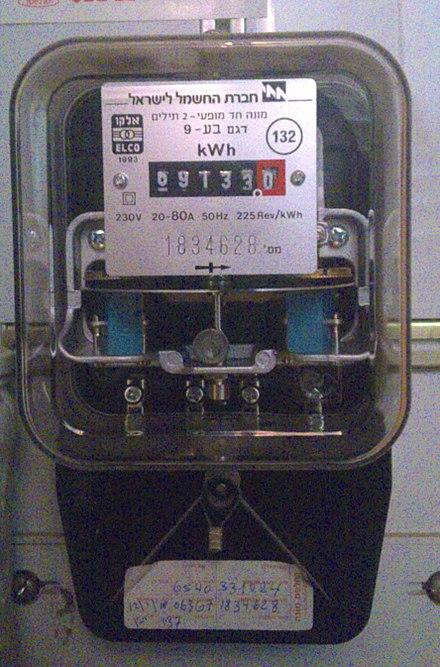
\includegraphics[scale=0.3]{meters.jpg}
	\caption{An Average Electricity Meter}
\end{figure}





\subsection{Measuring Electricity and Making of the Bill}
Power is first generated in a power plant after which Transmission high-voltage, i.e. $ 115 - 230kV $, is reduced to distribution-level voltage through transformers at a local distribution station. The lower voltage power is then transmitted to neighborhoods via distribution feeders, generally of a voltage on the order of $ 5 - 15 kV $, but can be as high as $ 34.5 kV $.
Voltage is again reduced to household-use level by pole-top or padmount transformers on the feeder, either $ 220/110 V $ or in some countries $ 440/220 V $, and carried into the home via service wires.

\subsubsection{Mains Power}
Mains Electricity or Domestic Power is a general-purpose alternating-current (AC) electric power supply. It is the form of electrical power that is delivered to homes and businesses through the electric grid in many parts of the world. People use this electricity to power everyday items—such as domestic appliances, televisions and lamps—by plugging them into a wall outlet.

The voltage and frequency of electric power differs between regions. In much of the world and India, a voltage (nominally) of 230 volts and frequency of 50 Hz is used. \textit{All voltages are root mean square voltage; the peak AC voltage is greater by a factor of $\sqrt{2}$, and the peak-to-peak voltage greater by a factor of $ 2\sqrt{2}. $}

\section{Methodology}

\subsection{Method of Calculation of Energy Consumed by Refrigerator}
Let us take an example of 340-liter refrigerator which is rated at 150 Watts with an operating hour of 24 hours. \\

\noindent
The Compressor Approximately runs for about 10 to 12 hours when outside Kitchen temperature is generally about 25 to 30 $\degree $ Centigrade. As the Dry Balcony door is generally open, and the Kitchen faces East, it is exposed to direct sunlight for about 8 hours, and has an elevated temperature in the first half of the day. \\

Per hour consumption of the Refrigerator while on Full power of the Compressor = 150 W\\

\noindent
While running with the compressor the Refrigerator consumes full wattage and without compressor, it consumes only $ 10 \% $ of the Total Wattage for minimal functioning.\\ 

Per day consumption will therefore be:
$$
\mathrm{(Hours\ Compressor\ is\ on)}\ \times\ 100\% \ \mathrm{Power}\ +\ \mathrm{(Hours\ Compressor\ is\ Off)}\ \times\ 10\%\ \mathrm{Power}
$$
\noindent
So, 
$$
\mathrm{Per\ Day\ Consumption\ } = 12 \times 130 + 12 \times 13 = 1716\ Wh = 1.71\ kWh
$$
\noindent
Therefore, 

$$
\mathrm{Per\ Month\ Consumption\ } = 1.71\ kWh \times 30 = \textbf{51.3\ kWh}
$$


\subsection{Method of Calculation of Energy Consumed by Air Conditioner}
The AC is switched on only on days when the temperature in the room is generally above 25 \degree Centigrade. The Thermostat on the AC is kept on 24 \degree Centigrade. So the compressor will run on full power until that temperature is reached which generally happens within 15 minutes, after which the AC is switched off. So the Compressor runs the entire time the AC is on. \\
\noindent
Wattage of the AC is 1800W. \\
Time used = 20 Minutes = 0.33 Hr\\
Days used = 6\\
Therefore, 
Power Consumed by the AC = Wattage $\times$ Time Used. 
$$
\mathrm{Per\ Month\ Consumption\ } = 1800W \times 0.33hr \times 6 = \textbf{7.128\ kWh}
$$
\subsection{Method of Calculation of Energy Consumed by Other Appliances}

For all Other Appliances, the method of calculation is standard and constant. Their wattage is checked, and is multiplied by the number of hours it has been used. \\

\noindent
Example of a Bulb:\\

\noindent
Power Rating in Watt: 10W\\
Number of Such Bulbs: 4\\
Number of Hours used: 7\\
Number of Days used: 30\\

Then Energy Consumed per Month = (Power) * (No. of Bulbs) * (No. of Hours) * (No. of Days)

$$
\mathrm{Per\ Month\ Consumption\ } = 10W \times 4 \times 7 \times 30 = \textbf{8.4\ kWh}
$$

It is calculated similarly for all the other electrical components. 
\pagebreak
\section{Observations}

\begin{tabularx}{1\textwidth} { 
		| >{\centering\arraybackslash}X 
		| >{\centering\arraybackslash}X 
		| >{\centering\arraybackslash}X 
		| >{\centering\arraybackslash}X 
		| >{\centering\arraybackslash}X 
		| >{\centering\arraybackslash}X 
		| >{\centering\arraybackslash}X | }
	\hline
	Sr.No & Power Rating (W) & Hours Used Per Day (Hr) & Days used & Number of Items & Energy  (kWh)\\
	\hline
	Bulb	&10	&7	&30	&4	&8.4	\\
	\hline
	Bulb	&10	&1	&30	&5	&1.5	\\
	\hline
	Tubelight	&20	&7	&30	&1	&4.2	\\
	\hline
	Phone Charger	&20	&3	&30	&3	&5.4	\\
	\hline
	Laptop Charger	&65	&15	&30	&2	&58.5	\\
	\hline
	Monitor	&20	&15	&30	&1	&9.0	\\
	\hline
	Monitor	&20	&9	&30	&1	&5.4	\\
	\hline
	Television	&80	&2	&30	&1	&4.8	\\
	\hline
	Refrigerator	&130	&24	&30	&1	&51.3	\\
	\hline
	Water Filter	&50	&1	&30	&1 &1.5	\\
	\hline
	Water Heater	&2000	&0.5	&20	&1	&20.0	\\
	\hline
	Air Conditioner	&1800	&0.33	&6	&2	&7.12	\\
	\hline
	Washing Machine	&450	&1	&30	&1	&13.5	\\
	\hline
	Fan	&60	&15	&30	&1	&27.0	\\
	\hline
	Fan	&50	&7	&30	&1	&10.5	\\
	\hline
	Fan	&45	&1	&30	&1	&1.3	\\
	\hline
\end{tabularx}
\vspace{5pt}\\\\
Therefore the Total Electrical Energy consumed is: \textbf{229.42 kWh = 229.42 Units}

\section{Calculations}

\subsection{Bulbs and Tubelights}
There are several bulbs in the house, and they are used at different times. The ones in Bedrooms are switched on for the most time, while the ones in the balcony and Bathrooms are switched on for very less times. \\

\noindent
\textit{For Bulbs in the Bedrooms and Kitchen :\\}

\noindent
Power Rating in Watt: 10W\\
Number of Such Bulbs: 4\\
Number of Hours used: 7\\
Number of Days used: 30\\

Then Energy Consumed per Month = (Power) * (No. of Bulbs) * (No. of Hours) * (No. of Days)

$$
\mathrm{Per\ Month\ Consumption\ } = 10 \times 4 \times 7 \times 30 = \textbf{8.4\ kWh}
$$

\noindent
\textit{For Bulbs in the Bathrooms, Balcony and Lobby:\\}

\noindent
Power Rating in Watt: 10W\\
Number of Such Bulbs: 5\\
Number of Hours used: 1\\
Number of Days used: 30\\

Then Energy Consumed per Month = (Power) * (No. of Bulbs) * (No. of Hours) * (No. of Days)

$$
\mathrm{Per\ Month\ Consumption\ } = 10 \times 5 \times 1 \times 30 = \textbf{1.5\ kWh}
$$

\noindent
\textit{For Tubelight in the Hall:\\
}

\noindent
Power Rating in Watt: 20W\\
Number of Such Tubelights: 1\\
Number of Hours used: 7\\
Number of Days used: 30\\

Then Energy Consumed per Month = (Power) * (No. of Tubelights) * (No. of Hours) * (No. of Days)

$$
\mathrm{Per\ Month\ Consumption\ } = 20 \times 1 \times 7 \times 30 = \textbf{4.2\ kWh}
$$

\underline{Total Energy Consumed by Bulbs and Tubelights: \textbf{14.1\ kWh}}

\subsection{Fans}
The Fans in the house are also used according to convenience. \\

\noindent
\textit{For the Fan in Bedroom 1: \\}

\noindent
Power Rating in Watt: 60W\\
Number of Such Fans: 1\\
Number of Hours used: 15\\
Number of Days used: 30\\

Then Energy Consumed per Month = (Power) * (No. of Fans) * (No. of Hours) * (No. of Days)

$$
\mathrm{Per\ Month\ Consumption\ } = 60 \times 1 \times 15 \times 30 = \textbf{27.00\ kWh}
$$

\noindent
\textit{For the Fan in Bedroom 2:\\}

\noindent
Power Rating in Watt: 50W\\
Number of Such Fans: 1\\
Number of Hours used: 7\\
Number of Days used: 30\\

Then Energy Consumed per Month = (Power) * (No. of Fans) * (No. of Hours) * (No. of Days)

$$
\mathrm{Per\ Month\ Consumption\ } = 50 \times 1 \times 7 \times 30 = \textbf{10.5\ kWh}
$$


\noindent
\textit{For the Fan in the Hall: \\}

\noindent
Power Rating in Watt: 45W\\
Number of Such Fans: 1\\
Number of Hours used: 7\\
Number of Days used: 30\\

Then Energy Consumed per Month = (Power) * (No. of Fans) * (No. of Hours) * (No. of Days)

$$
\mathrm{Per\ Month\ Consumption\ } = 45 \times 1 \times 1 \times 30 = \textbf{1.3\ kWh}
$$

\underline{Total Energy Consumed by Fans: \textbf{38.8\ kwH}}


\subsection{Chargers}
Since the beginning of working from home, Heavy Laptop chargers are under constant use, while lighter Phone chargers with fast charging are relatively low powered. \\

\noindent
\textit{For Laptop Chargers:\\}

\noindent
Power Rating in Watt: 65W\\
Number of Such Chargers: 2\\
Number of Hours used: 15\\
Number of Days used: 30\\

Then Energy Consumed per Month = (Power) * (No. of Chargers) * (No. of Hours) * (No. of Days)

$$
\mathrm{Per\ Month\ Consumption\ } = 65 \times 2 \times 15 \times 30 = \textbf{58.5\ kWh}
$$

\noindent
\textit{For Phone Chargers:\\}

\noindent
Power Rating in Watt: 20W\\
Number of Such Chargers: 3\\
Number of Hours used: 3\\
Number of Days used: 30\\

Then Energy Consumed per Month = (Power) * (No. of Chargers) * (No. of Hours) * (No. of Days)

$$
\mathrm{Per\ Month\ Consumption\ } = 20 \times 3 \times 3 \times 30 = \textbf{5.4\ kWh}
$$

\underline{Total Energy Consumed by Chargers: \textbf{63.9\ kWh}}

\subsection{Monitors}
Two monitors are used connected to laptops, that are used at different time intervals. The Monitors 24'' LED backlit and therefore are energy efficient. 

\noindent
Power Rating in Watt: 20W\\
Number of Such Monitors: 1\\
Number of Hours used: 15\\
Number of Days used: 30\\

Then Energy Consumed per Month = (Power) * (No. of Monitors) * (No. of Hours) * (No. of Days)

$$
\mathrm{Per\ Month\ Consumption\ } = 20 \times 1 \times 15 \times 30 = \textbf{9.0\ kWh}
$$

\noindent
Power Rating in Watt: 20W\\
Number of Such Monitors: 1\\
Number of Hours used: 8\\
Number of Days used: 30\\

Then Energy Consumed per Month = (Power) * (No. of Monitors) * (No. of Hours) * (No. of Days)

$$
\mathrm{Per\ Month\ Consumption\ } = 20 \times 1 \times 8 \times 30 = \textbf{4.8\ kWh}
$$

\underline{Total Energy Consumed by Monitors: \textbf{13.8\ kWh}}

\subsection{Television}

\noindent
Power Rating in Watt: 80W\\
Number of Such TVs: 1\\
Number of Hours used: 2\\
Number of Days used: 30\\

Then Energy Consumed per Month = (Power) * (No. of TV) * (No. of Hours) * (No. of Days)

$$
\mathrm{Per\ Month\ Consumption\ } = 80 \times 1 \times 2 \times 30 = \textbf{4.8\ kWh}
$$


\subsection{Refrigerator}
Per hour consumption of the Refrigerator while on Full power of the Compressor = 150 W\\

\noindent
While running with the compressor the Refrigerator consumes full wattage and without compressor, it consumes only $ 10 \% $ of the Total Wattage for minimal functioning.\\ 

Per day consumption will therefore be:
$$
\mathrm{(Hours\ Compressor\ is\ on)}\ \times\ 100\% \ \mathrm{Power}\ +\ \mathrm{(Hours\ Compressor\ is\ Off)}\ \times\ 10\%\ \mathrm{Power}
$$
\noindent
So, 
$$
\mathrm{Per\ Day\ Consumption\ } = 12 \times 130 + 12 \times 13 = 1716\ Wh = 1.71\ kWh
$$
\noindent
Therefore, 

$$
\mathrm{Per\ Month\ Consumption\ } = 1.71\ kWh \times 30 = \textbf{51.3\ kWh}
$$

\subsection{Air Conditioners}
The AC is switched on only on days when the temperature in the room is generally above 25 \degree Centigrade. The Thermostat on the AC is kept on 24 \degree Centigrade. So the compressor will run on full power until that temperature is reached which generally happens within 15 minutes, after which the AC is switched off. So the Compressor runs the entire time the AC is on. \\
\noindent
Wattage of the AC is 1800W. \\
Time used = 20 Minutes = 0.33 Hr\\
Days used = 6\\
Therefore, 
Power Consumed by the AC = Wattage $\times$ Time Used. 
$$
\mathrm{Per\ Month\ Consumption\ } = 1800W \times 0.33hr \times 6 = \textbf{7.128\ kWh}
$$
\subsection{Water Heater}
Water heater is used occasionally as Solar heated water is available from the Building. \\

\noindent
Power Rating in Watt: 2000W\\
Number of Such Heaters: 1\\
Number of Hours used: 0.5\\
Number of Days used: 20\\

Then Energy Consumed per Month = (Power) * (No. of Heaters) * (No. of Hours) * (No. of Days)

$$
\mathrm{Per\ Month\ Consumption\ } = 2000 \times 1 \times 0.5 \times 20 = \textbf{20.0\ kWh}
$$

\subsection{Water Filter}
\noindent
Power Rating in Watt: 50W\\
Number of Such Filters: 1\\
Number of Hours used: 1\\
Number of Days used: 30\\

Then Energy Consumed per Month = (Power) * (No. of Filters) * (No. of Hours) * (No. of Days)

$$
\mathrm{Per\ Month\ Consumption\ } = 50 \times 1 \times 1 \times 30 = \textbf{1.5\ kWh}
$$

\subsection{Washing Machine}

\noindent
Power Rating in Watt: 450W\\
Number of Such Washing Machines: 1\\
Number of Hours used: 1\\
Number of Days used: 30\\

Then Energy Consumed per Month = (Power) * (No. of Washing Machines) * (No. of Hours) * (No. of Days)

$$
\mathrm{Per\ Month\ Consumption\ } = 450 \times 1 \times 1 \times 30 = \textbf{13.5\ kWh}
$$


\section{Results}

\subsection{Electricity Bill and Meter Reading}
\begin{figure}[H]
	\centering
	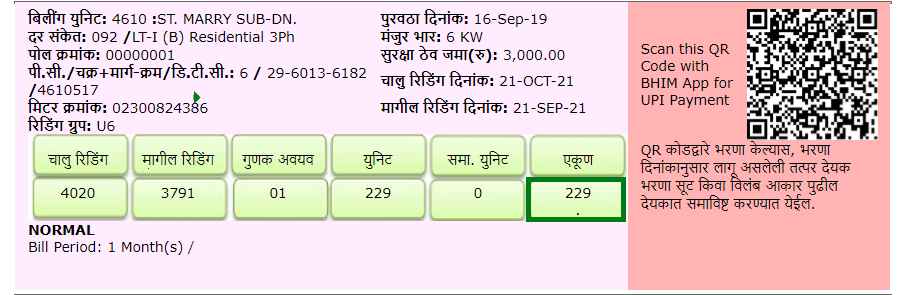
\includegraphics[scale=0.74]{bill.png}
	\caption{Amount in Units}
\end{figure}

\begin{figure}[H]
	\centering
	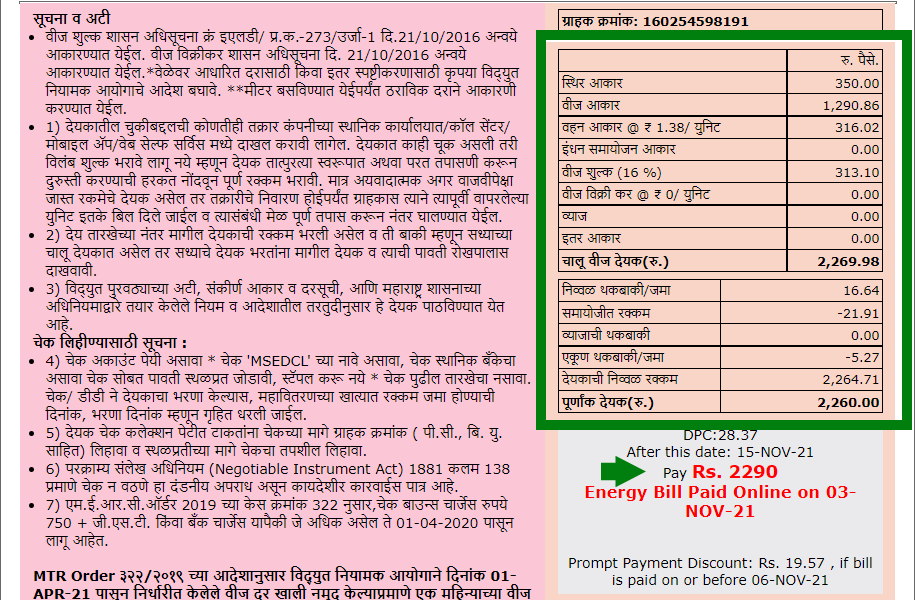
\includegraphics[scale=0.7]{bill 2.png}
	\caption{Breakdown of Payable Amount}
\end{figure}

\begin{figure}[H]
	\centering
	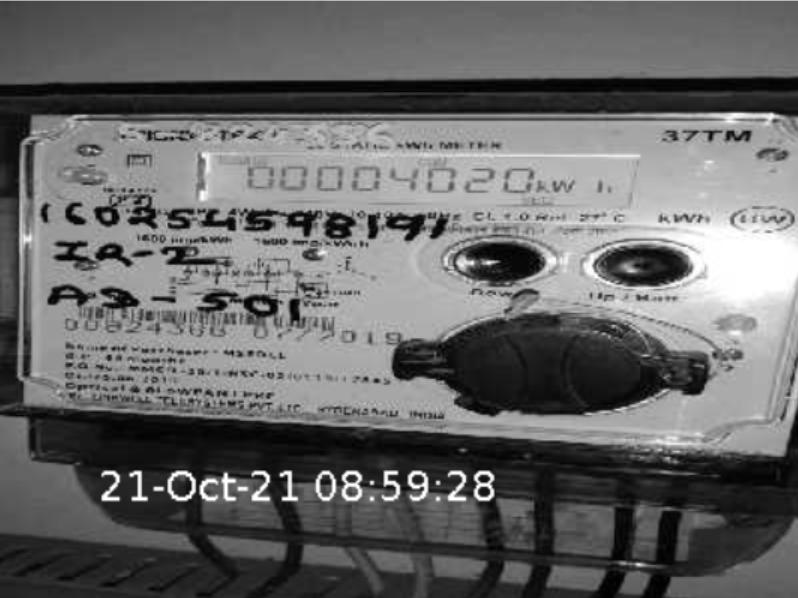
\includegraphics[scale=0.3]{meter.jpg}
	\caption{Reading from the Meter, Provided by Government on Website for each Invoice}
\end{figure}

\subsection{Theoretically Calculated Value}

\begin{figure}[H]
	\centering
	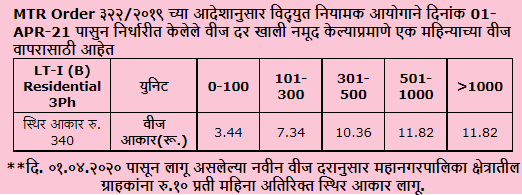
\includegraphics[scale=0.7]{Unit Price Slabs.png}
	\caption{Unit Slabs per Price}
\end{figure}


\noindent
Number of Units Calculated Theoretically\hfill: \textbf{229.42}\\
Price in Rupees for first 100 units\hfill: \textbf{3.44} Rs.\\
Price in Rupees for 100 to 300 units\hfill: \textbf{7.34} Rs. \\
\noindent
Therefore, Total Price of Electricity alone is: \\

(Price for first 100) * 100 + (Price for 100 to 300) * (Remaining Units)\\

\noindent
Remaining Units: 229.42 - 100 = 129.42\\
Total Price = 
$$
3.44 \times 100\ +\  7.34 \times 129.42\ = \textbf{1293.94 Rs. }
$$

\noindent
Base Electricity Charge \hfill = 350 Rs.\\
Transport Charge 		= 1.38 Rs per Unit = $ 1.38 \times 229.42  \hfill= 316.59 Rs. $\\
Total 					\hfill= 1960.53 Rs.\\
Electricity Tax (16\%)	= 16\% of 1960.53 Rs \hfill= 313.68 Rs.\\
Total Amount 			= 313.68 + 1960.53 Rs \hfill= \textbf{2274.21 Rs. }
						
\subsection{Net Error Percentage}
Theoretically Calculated Energy Consumed 	\hfill= \textbf{229.42 kWh}\\
Amount on Electricity Bill 					\hfill= \textbf{229.00 kWh}\\

\noindent
Theoretically Calculated Amount	\hfill= \textbf{2274.21 Rs. }\\
Actual Bill Amount				\hfill= \textbf{2260.00 Rs. }

$$ \mathrm{Error} = \dfrac{|\mathrm{Real\ Value} - \mathrm{Observed\ value}|}{\mathrm{Real\ Value}}$$

$$\eta = \frac{|2260.00 - 2274.21|}{2260.00} = 0.01 \%$$

\section{Conclusion}

The Energy requirements of a Flat were audited with an error of 0.01\%. The concepts and methodologies involved were thoroughly understood and studied. The Main components that consume electricity were found to be 65 W Laptop Chargers, the Refrigerator and the Fans.\\

Over the Last year, a spike in the Electricity Bill had been noticed as compared to pre-Lockdown times, and it is not clear that due to work from Home, our use of Computers has dramatically increased resulting in an increased Electricity bill. It is hoped that once work is offline again, the power bill must drop to about Two Thirds of its current amount. \\

Some Places where Power could certainly be saved are the Fans. Bulbs used significantly less power compared to all other applicances due to their efficiency, and therefore it is more feasable to keep a bulb on for the entire night rather than a laptop charger or a Monitor. The Bill from the Laptops can also be reduced by unplugging it and using it on battery until it is drained rather than keeping it constantly connected. 

\end{document}